
\newpage
\setlength{\voffset}{-3cm}

\begin{center}
\section{\textbf{\huge{Form}}}

\Large{Use Cases}
\end{center}

%--------START EDITING HERE FOR HANDLING---------
%Maria

%--------Form Use case---------
\subsection{addNewForm}
\textbf{Description:}
This use-case allows for the addition of a new form on to the system.
\subsubsection{Prioritization:}
Nice-to-Have
\subsubsection{Conditions and Data Structures:}
\textbf{Pre-Conditions:}
\begin{itemize}
	\item User has Administrator rights on the system.
	\item Form must not exist on the system.
\end{itemize}

\textbf{Post-Conditions:}	
\begin{itemize}
	\item New form is created and persisted to Database
\end{itemize}
\subsubsection{Service Contract:} 
%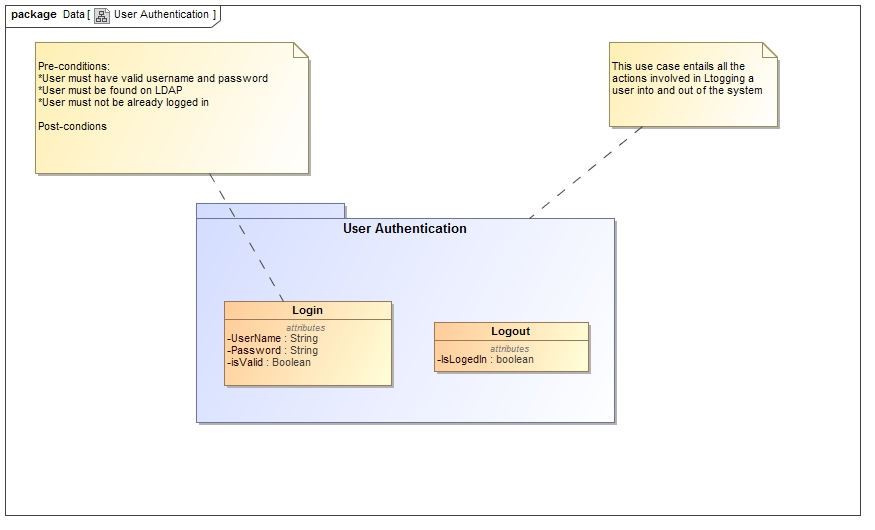
\includegraphics[width=1\linewidth]{./Images/Author/Login.jpg}\\
\subsubsection{Required Functionality:}
\subsubsection{Process Specifications:} 

%\textbf{Use case diagram for Login}\\
%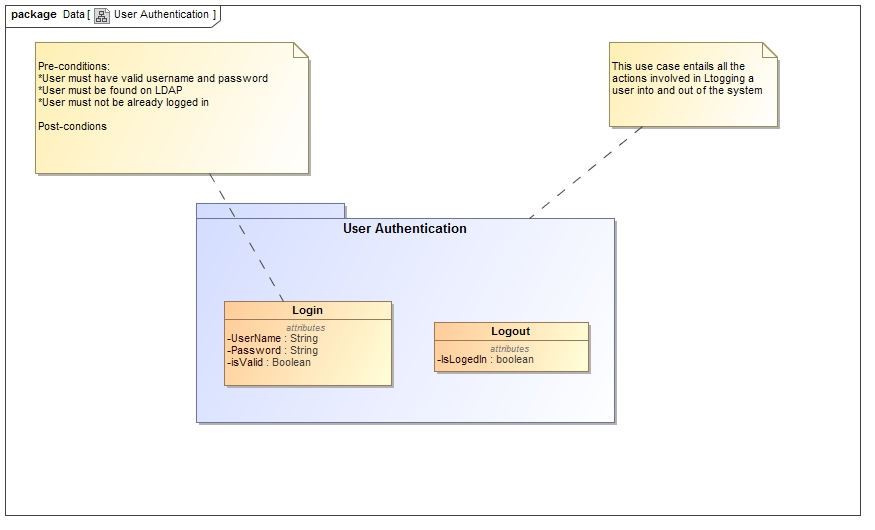
\includegraphics[width=1\linewidth]{./Images/Author/Login.jpg}\\


viewForm(String Patient name)	
Pre Form must exist
Pre Patient must exist.	
Post View a specific form for a patient
\subsection{viewForm}
\textbf{Description:}
This use-case allows for viewing of a form for a particular patient.
\subsubsection{Prioritization:}
Important
\subsubsection{Conditions and Data Structures:}
\textbf{Pre-Conditions:}
\begin{itemize}
	\item Form must exist
	\item Patient must exist.
\end{itemize}

\textbf{Post-Conditions:}	
\begin{itemize}
	\item Patient Form is displayed on GUI
\end{itemize}
\subsubsection{Service Contract:} 
%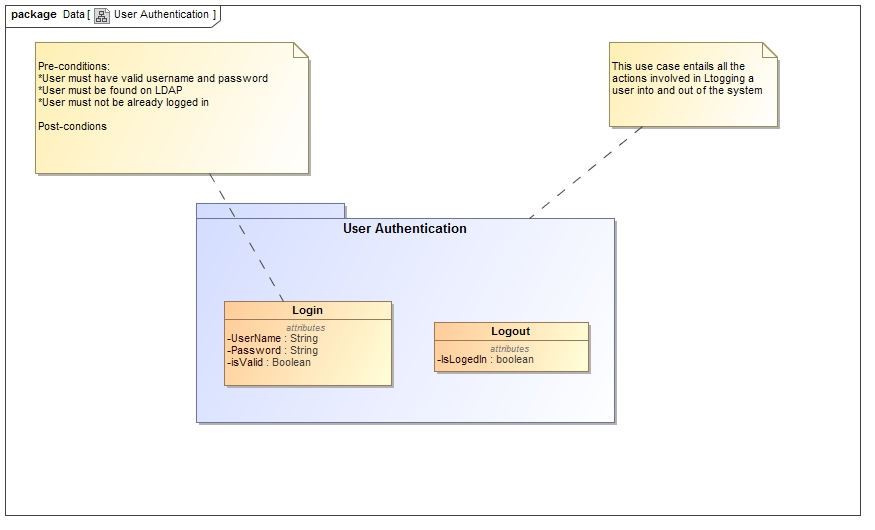
\includegraphics[width=1\linewidth]{./Images/Author/Login.jpg}\\
\subsubsection{Required Functionality:} 
\subsubsection{Process Specifications:} 

%\textbf{Use case diagram for Login}\\
%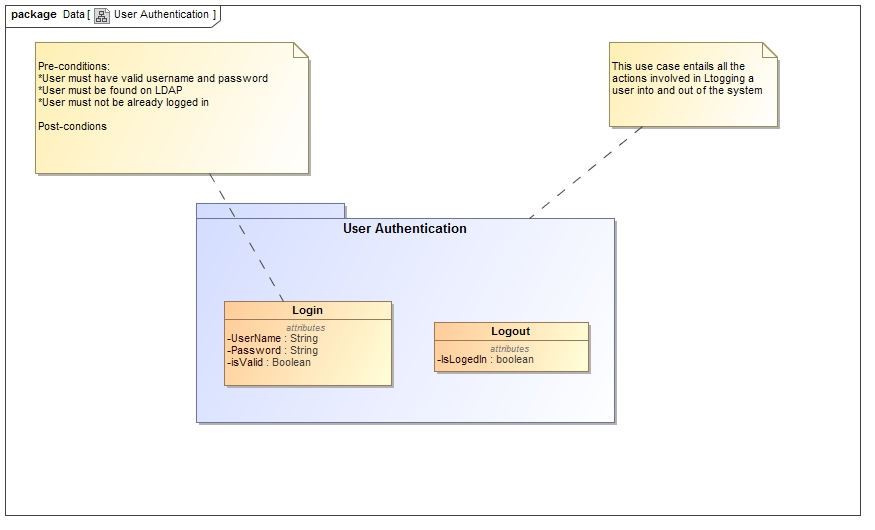
\includegraphics[width=1\linewidth]{./Images/Author/Login.jpg}\\




removeForm(String form name)	
Pre Form must exist. 
Pre No data must be present in the form.	
Post Form is deleted from DB

\subsection{removeForm}
\textbf{Description:}
This use-case allows for the logical removal of a form in that the form will be archived on the system so that it can be retrieved later if needed.
\subsubsection{Prioritization:}
Important
\subsubsection{Conditions and Data Structures:}
\textbf{Pre-Conditions:}
\begin{itemize}
	\item User has Administrator rights on the system.
	\item Form to be removed must exist.
	\item The editable form fields must not be filled in at time for deletion
\end{itemize}

\textbf{Post-Conditions:}	
\begin{itemize}
	\item Form is archived
\end{itemize}
\subsubsection{Service Contract:} 
%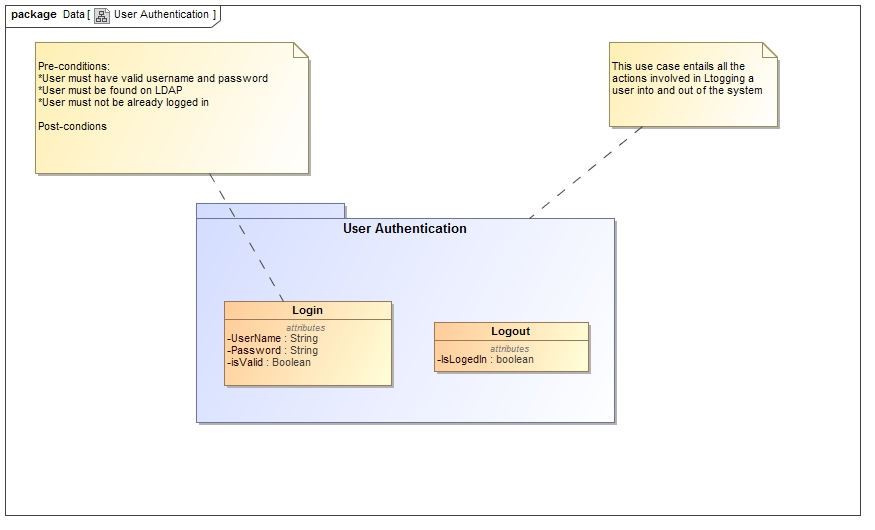
\includegraphics[width=1\linewidth]{./Images/Author/Login.jpg}\\
\subsubsection{Required Functionality:} 
\subsubsection{Process Specifications:} 

%\textbf{Use case diagram for Login}\\
%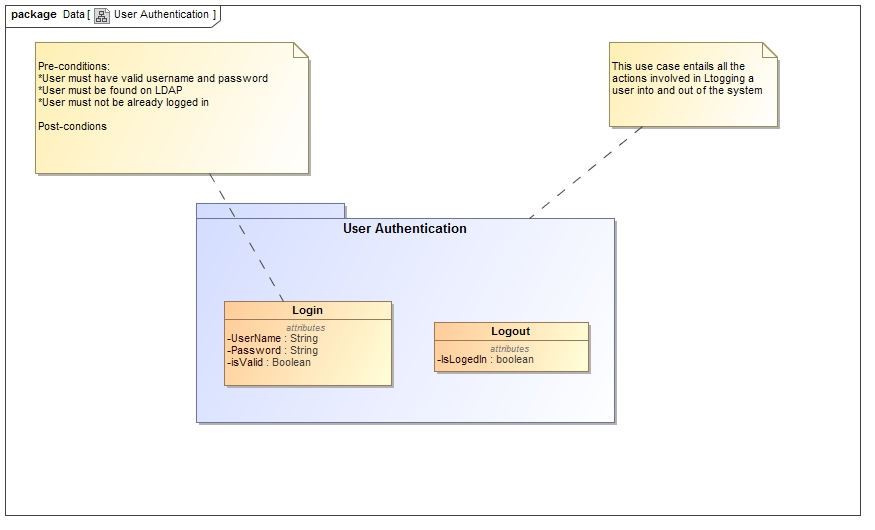
\includegraphics[width=1\linewidth]{./Images/Author/Login.jpg}\\





addFormFields()
i.e. add more fields to an existing form	
Pre Form must exist	
Post Field is added to GUI and persisted to DB


\subsection{addFormField}
\textbf{Description:}
This use-case allows for the addition of a new form field into a currently existing form
\subsubsection{Prioritization:}
Nice-to-Have
\subsubsection{Conditions and Data Structures:}
\textbf{Pre-Conditions:}
\begin{itemize}
	\item User has Administrator rights on the system.
	\item Form must not exist on the system.
\end{itemize}

\textbf{Post-Conditions:}	
\begin{itemize}
	\item New form is created and persisted to Database
\end{itemize}
\subsubsection{Service Contract:} 
%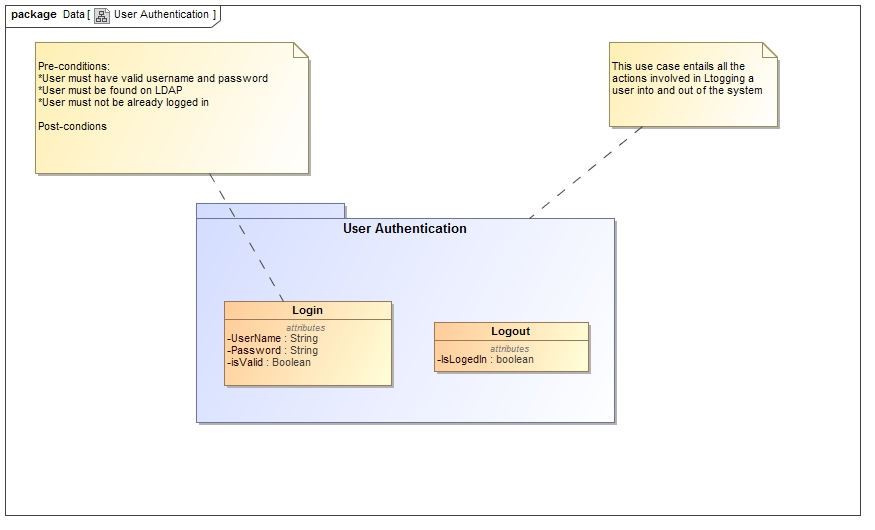
\includegraphics[width=1\linewidth]{./Images/Author/Login.jpg}\\
\subsubsection{Required Functionality:} 
\subsubsection{Process Specifications:} 

%\textbf{Use case diagram for Login}\\
%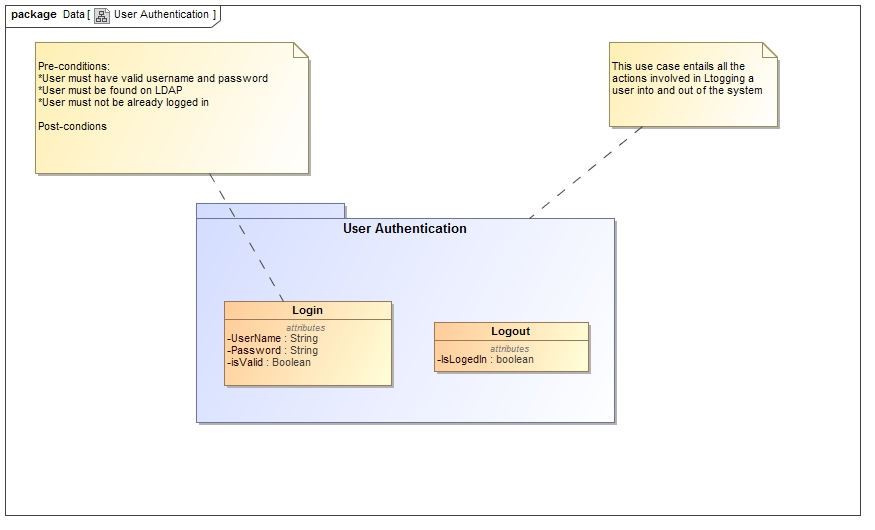
\includegraphics[width=1\linewidth]{./Images/Author/Login.jpg}\\



editFormFields(String form name)
i.e. 
being able to add to or remove from an existing form field	
Pre Field must exist. 
	Form must exist	
Post Edited field is updated on Form GUI and updated in DB

\subsection{editFormField}
\textbf{Description:}
This use-case allows for the editing of the field of a specific form that is on the system.
\subsubsection{Prioritization:}
Nice-to-Have
\subsubsection{Conditions and Data Structures:}
\textbf{Pre-Conditions:}
\begin{itemize}
	\item User has Administrator rights on the system.
	\item Field must exist on form.
\end{itemize}

\textbf{Post-Conditions:}	
\begin{itemize}
	\item Edited field is updated on Form GUI and updated in Database
\end{itemize}
\subsubsection{Service Contract:} 
%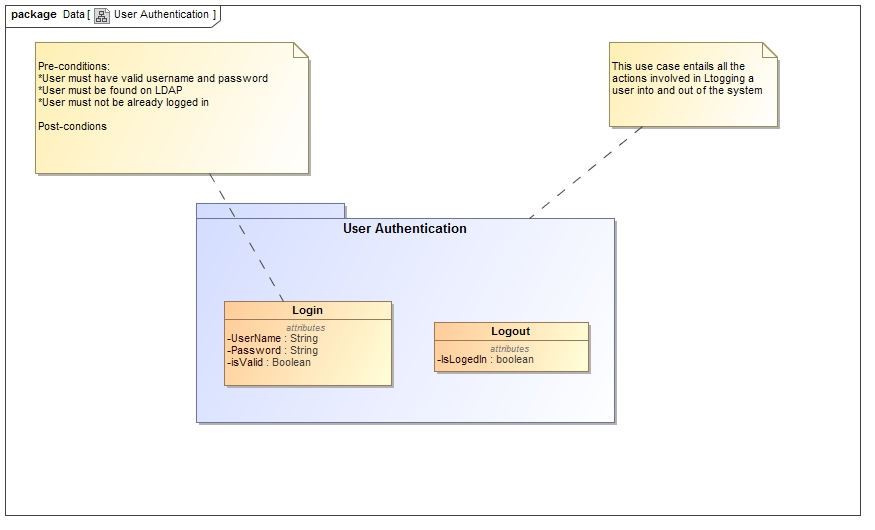
\includegraphics[width=1\linewidth]{./Images/Author/Login.jpg}\\
\subsubsection{Required Functionality:} 
\subsubsection{Process Specifications:} 

%\textbf{Use case diagram for Login}\\
%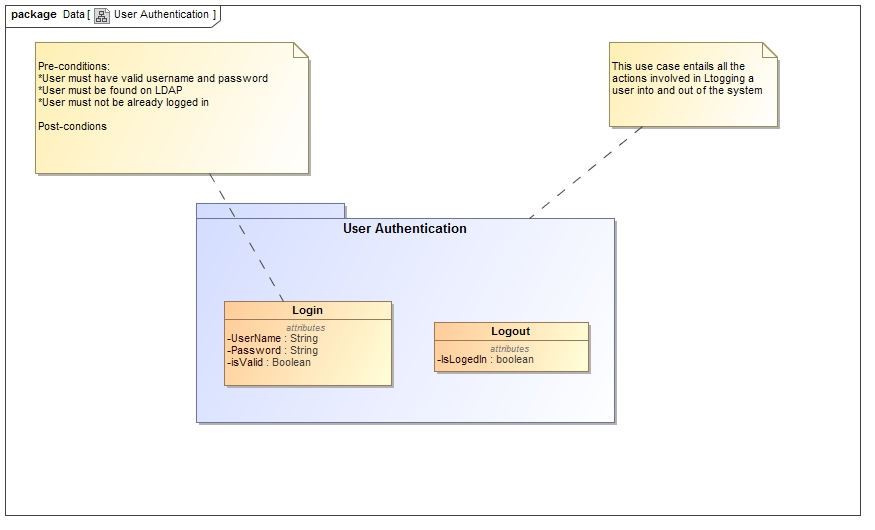
\includegraphics[width=1\linewidth]{./Images/Author/Login.jpg}\\



deleteFormFields()	
Pre Form must exist	
Post Field is removed from GUI and  persisted to DB

\subsection{deleteFormField}
\textbf{Description:}
This use-case allows for the logical deletion of a form field in that the field will no longer be shown on the GUI but would still be present in the Database.
\subsubsection{Prioritization:}
Nice-to-Have
\subsubsection{Conditions and Data Structures:}
\textbf{Pre-Conditions:}
\begin{itemize}
	\item User has Administrator rights on the system.
	\item Form must exist on the system.
\end{itemize}

\textbf{Post-Conditions:}	
\begin{itemize}
	\item Field is removed from GUI  
\end{itemize}
\subsubsection{Service Contract:} 
%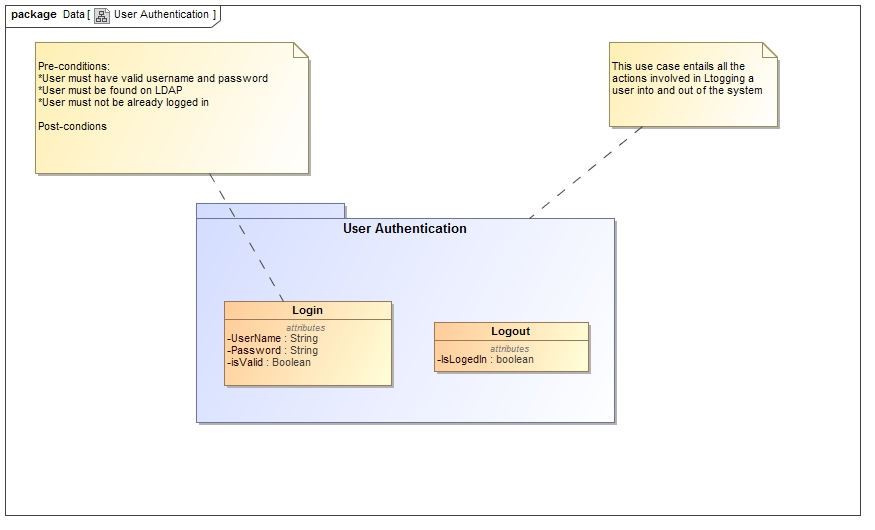
\includegraphics[width=1\linewidth]{./Images/Author/Login.jpg}\\
\subsubsection{Required Functionality:} 
\subsubsection{Process Specifications:} 

%\textbf{Use case diagram for Login}\\
%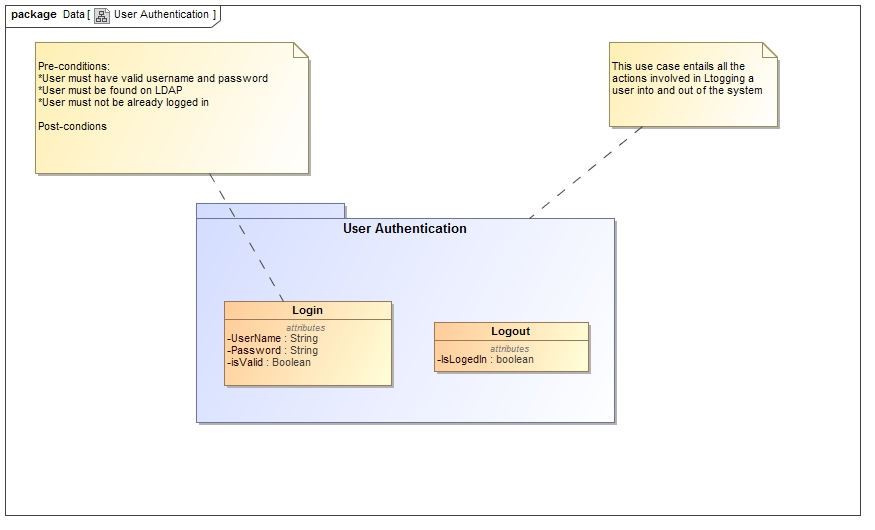
\includegraphics[width=1\linewidth]{./Images/Author/Login.jpg}\\



downloadPatientForm(String patient name,  String form name)
i.e. to download a specific form for a patient
Pre Patient information must exist, that is there must be information on that patient in the database.
	Form must exist.
	Patient must exist in DB.	
Post Form is downloaded from server to local hard drive

\subsection{downloadPatientForm} %for a specific form
\textbf{Description:}
This use-case allows for downloading of a particular form associated with the specified patient.
\subsubsection{Prioritization:}
Nice-to-Have
\subsubsection{Conditions and Data Structures:}
\textbf{Pre-Conditions:}
\begin{itemize}
	\item User has Administrator rights on the system.
	\item Form must exist on the system.
	\item Patient must exist on LDAP.
\end{itemize}

\textbf{Post-Conditions:}	
\begin{itemize}
	\item Forms are zipped and downloaded from server to local hard drive of user
\end{itemize}
\subsubsection{Service Contract:} 
%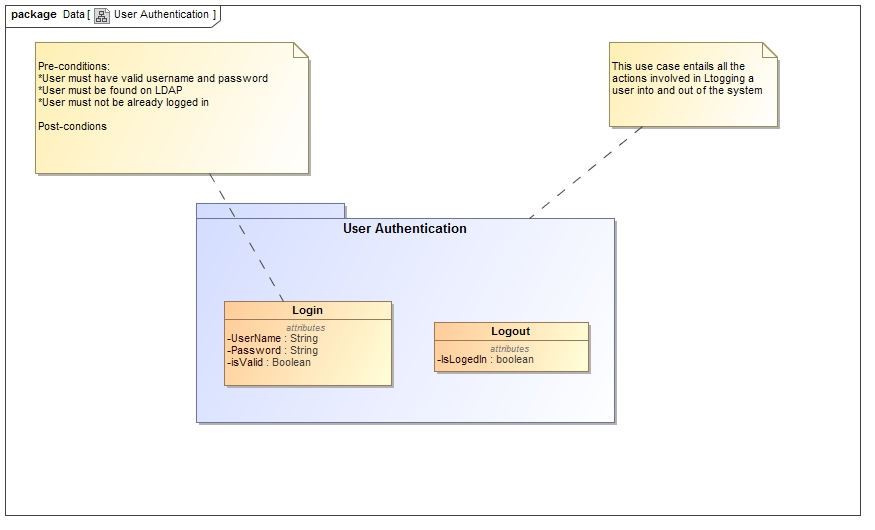
\includegraphics[width=1\linewidth]{./Images/Author/Login.jpg}\\
\subsubsection{Required Functionality:} 
\subsubsection{Process Specifications:}

%\textbf{Use case diagram for Login}\\
%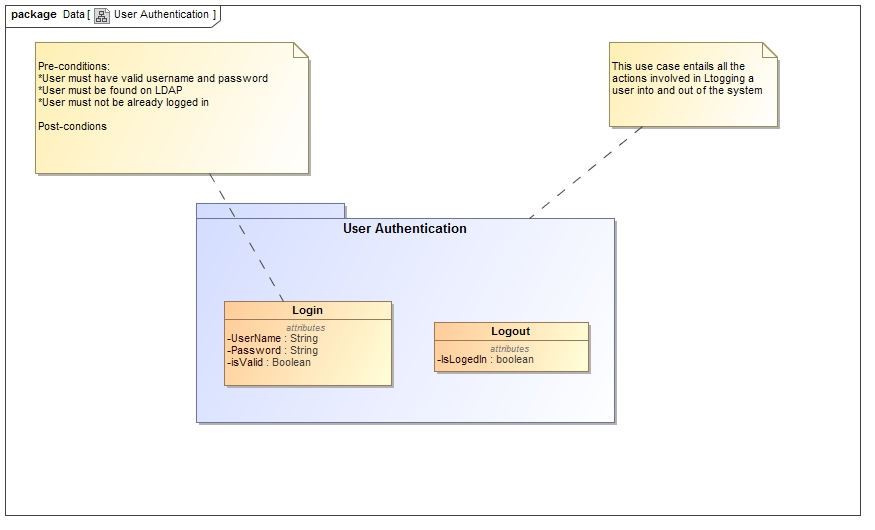
\includegraphics[width=1\linewidth]{./Images/Author/Login.jpg}\\



downloadPatientForms(String patient name) 
i.e. download all forms for a patient	
Pre Patient information must exist.
	Patient must exist on LDAP.	
Post Form is downloaded from server to user's local hard drive (in zipped format)


\subsection{downloadPatientForms} %download all forms
\textbf{Description:}
This use-case allows for downloading of all forms associated with the specified patient.
\subsubsection{Prioritization:}
Nice-to-Have
\subsubsection{Conditions and Data Structures:}
\textbf{Pre-Conditions:}
\begin{itemize}
	\item User has Administrator rights on the system.
	\item Form must exist on the system.
	\item Patient must exist on LDAP.
	\item Patient information must exist.
\end{itemize}

\textbf{Post-Conditions:}	
\begin{itemize}
	\item Form is downloaded from server to local hard drive of user
\end{itemize}
\subsubsection{Service Contract:} 
%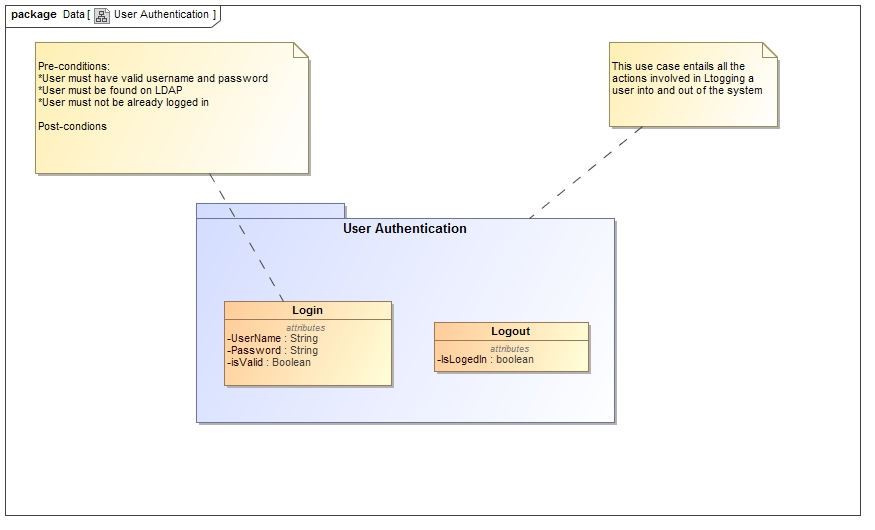
\includegraphics[width=1\linewidth]{./Images/Author/Login.jpg}\\
\subsubsection{Required Functionality:} 
\subsubsection{Process Specifications:} 

%\textbf{Use case diagram for Login}\\
%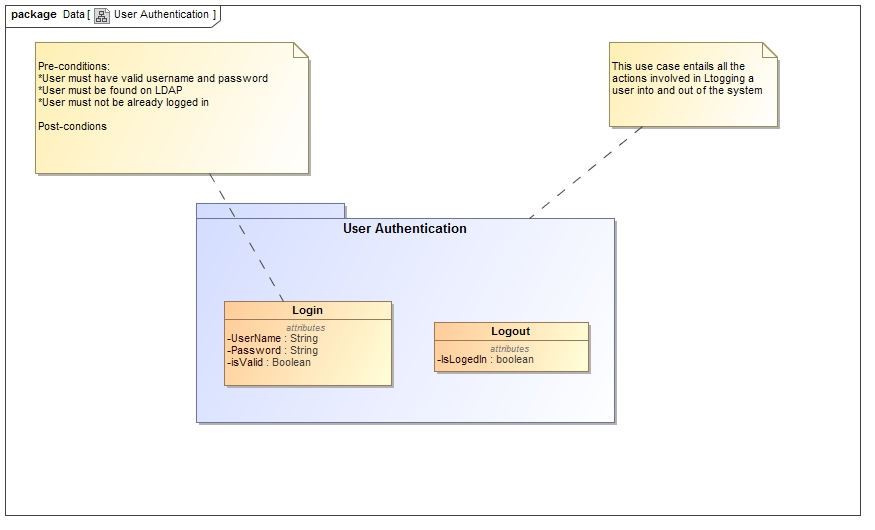
\includegraphics[width=1\linewidth]{./Images/Author/Login.jpg}\\




